\documentclass{standalone}
\usepackage{tikz}
\usetikzlibrary{patterns, positioning}
\usepackage[sfdefault]{ClearSans} %% option 'sfdefault' activates Clear Sans as the default text font
\usepackage[T1]{fontenc}

\begin{document}
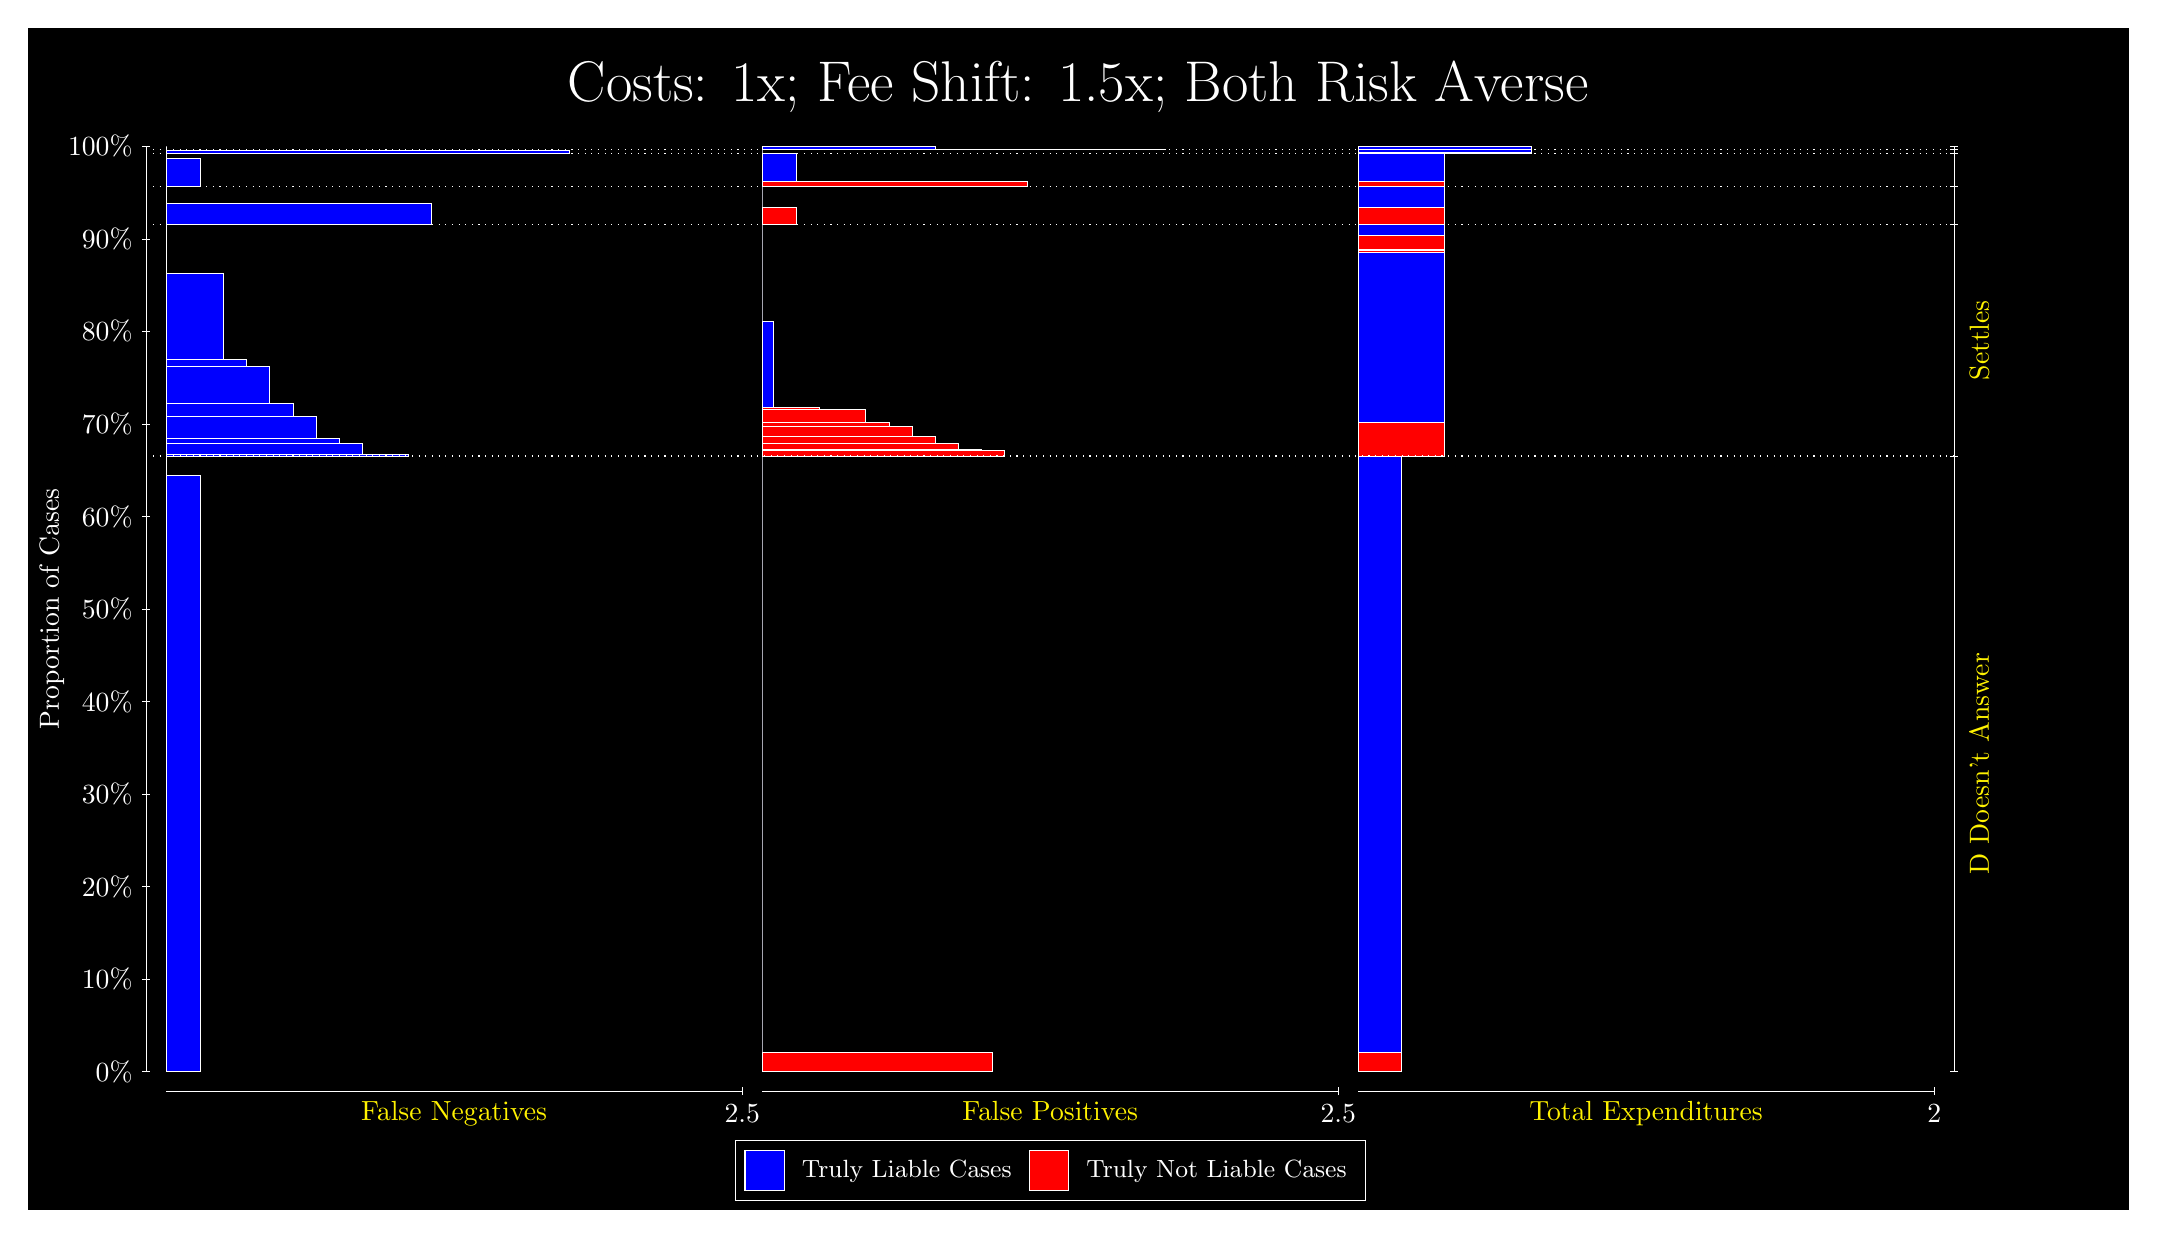
\begin{tikzpicture}
\draw[fill=black] (0,0) rectangle (26.667,15);
\draw[text=white] (0,13.5) rectangle (26.667,15) node[midway] {\huge Costs: 1x; Fee Shift: 1.5x; Both Risk Averse};
\draw[white, very thin] (1.5,1.75) -- (1.5,13.5);
\node[rotate=90, text=white, anchor=center] at (0.3, 7.625) {Proportion of Cases};
\draw[white, very thin] (1.45,1.75) -- (1.55,1.75);
\node[text=white, anchor=east] at (1.45, 1.75) {0\%};
\draw[white, very thin] (1.45,2.925) -- (1.55,2.925);
\node[text=white, anchor=east] at (1.45, 2.925) {10\%};
\draw[white, very thin] (1.45,4.1) -- (1.55,4.1);
\node[text=white, anchor=east] at (1.45, 4.1) {20\%};
\draw[white, very thin] (1.45,5.275) -- (1.55,5.275);
\node[text=white, anchor=east] at (1.45, 5.275) {30\%};
\draw[white, very thin] (1.45,6.45) -- (1.55,6.45);
\node[text=white, anchor=east] at (1.45, 6.45) {40\%};
\draw[white, very thin] (1.45,7.625) -- (1.55,7.625);
\node[text=white, anchor=east] at (1.45, 7.625) {50\%};
\draw[white, very thin] (1.45,8.8) -- (1.55,8.8);
\node[text=white, anchor=east] at (1.45, 8.8) {60\%};
\draw[white, very thin] (1.45,9.975) -- (1.55,9.975);
\node[text=white, anchor=east] at (1.45, 9.975) {70\%};
\draw[white, very thin] (1.45,11.15) -- (1.55,11.15);
\node[text=white, anchor=east] at (1.45, 11.15) {80\%};
\draw[white, very thin] (1.45,12.325) -- (1.55,12.325);
\node[text=white, anchor=east] at (1.45, 12.325) {90\%};
\draw[white, very thin] (1.45,13.5) -- (1.55,13.5);
\node[text=white, anchor=east] at (1.45, 13.5) {100\%};

\draw[white, very thin] (24.457,1.75) -- (24.457,13.5);
\draw[white, very thin] (24.407,1.75) -- (24.507,1.75);
\node[anchor=west] at (24.407, 1.75) {};
\draw[white, very thin] (24.407,9.5668) -- (24.507,9.5668);
\node[anchor=west] at (24.407, 9.5668) {};
\draw[white, very thin] (24.407,12.509) -- (24.507,12.509);
\node[anchor=west] at (24.407, 12.509) {};
\draw[white, very thin] (24.407,12.993) -- (24.507,12.993);
\node[anchor=west] at (24.407, 12.993) {};
\draw[white, very thin] (24.407,13.413) -- (24.507,13.413);
\node[anchor=west] at (24.407, 13.413) {};
\draw[white, very thin] (24.407,13.46) -- (24.507,13.46);
\node[anchor=west] at (24.407, 13.46) {};
\draw[white, very thin] (24.407,13.5) -- (24.507,13.5);
\node[anchor=west] at (24.407, 13.5) {};

\draw[white, very thin, fill=blue] (1.75,1.75) rectangle (2.1891,9.3207);
\draw[white, very thin, fill=red] (1.75,9.3207) rectangle (1.75,9.5668);
\draw[white, very thin, fill=blue] (1.75,9.5668) rectangle (4.8239,9.584);
\draw[white, very thin, fill=blue] (1.75,9.584) rectangle (4.2384,9.7258);
\draw[white, very thin, fill=blue] (1.75,9.7258) rectangle (3.9457,9.7931);
\draw[white, very thin, fill=blue] (1.75,9.7931) rectangle (3.6529,10.075);
\draw[white, very thin, fill=blue] (1.75,10.075) rectangle (3.3602,10.242);
\draw[white, very thin, fill=blue] (1.75,10.242) rectangle (3.0674,10.703);
\draw[white, very thin, fill=blue] (1.75,10.703) rectangle (2.7746,10.8);
\draw[white, very thin, fill=blue] (1.75,10.8) rectangle (2.4819,11.887);
\draw[white, very thin, fill=red] (1.75,11.887) rectangle (1.75,12.509);
\draw[white, very thin, fill=blue] (1.75,12.509) rectangle (5.1167,12.771);
\draw[white, very thin, fill=red] (1.75,12.771) rectangle (1.75,12.993);
\draw[white, very thin, fill=blue] (1.75,12.993) rectangle (2.1891,13.345);
\draw[white, very thin, fill=red] (1.75,13.345) rectangle (1.75,13.413);
\draw[white, very thin, fill=blue] (1.75,13.413) rectangle (6.8732,13.447);
\draw[white, very thin, fill=red] (1.75,13.447) rectangle (1.75,13.46);
\draw[white, very thin, fill=red] (1.75,13.46) rectangle (1.75,13.464);
\draw[white, very thin, fill=blue] (1.75,13.464) rectangle (1.75,13.5);
\draw[white, very thin, fill=red] (9.3189,1.75) rectangle (12.246,1.9961);
\draw[white, very thin, fill=blue] (9.3189,1.9961) rectangle (9.3189,9.5668);
\draw[white, very thin, fill=red] (9.3189,9.5668) rectangle (12.393,9.6348);
\draw[white, very thin, fill=red] (9.3189,9.6348) rectangle (12.1,9.6527);
\draw[white, very thin, fill=red] (9.3189,9.6527) rectangle (11.807,9.7341);
\draw[white, very thin, fill=red] (9.3189,9.7341) rectangle (11.515,9.8164);
\draw[white, very thin, fill=red] (9.3189,9.8164) rectangle (11.222,9.9475);
\draw[white, very thin, fill=red] (9.3189,9.9475) rectangle (10.929,9.9939);
\draw[white, very thin, fill=red] (9.3189,9.9939) rectangle (10.929,9.9952);
\draw[white, very thin, fill=red] (9.3189,9.9952) rectangle (10.636,10.166);
\draw[white, very thin, fill=red] (9.3189,10.166) rectangle (10.051,10.189);
\draw[white, very thin, fill=blue] (9.3189,10.189) rectangle (9.4652,11.276);
\draw[white, very thin, fill=blue] (9.3189,11.276) rectangle (9.3189,12.509);
\draw[white, very thin, fill=red] (9.3189,12.509) rectangle (9.758,12.731);
\draw[white, very thin, fill=blue] (9.3189,12.731) rectangle (9.3189,12.993);
\draw[white, very thin, fill=red] (9.3189,12.993) rectangle (12.686,13.061);
\draw[white, very thin, fill=blue] (9.3189,13.061) rectangle (9.758,13.413);
\draw[white, very thin, fill=red] (9.3189,13.413) rectangle (9.3189,13.426);
\draw[white, very thin, fill=blue] (9.3189,13.426) rectangle (9.3189,13.46);
\draw[white, very thin, fill=red] (9.3189,13.46) rectangle (14.442,13.464);
\draw[white, very thin, fill=blue] (9.3189,13.464) rectangle (11.515,13.5);
\draw[white, very thin, fill=red] (16.888,1.75) rectangle (17.437,1.9961);
\draw[white, very thin, fill=blue] (16.888,1.9961) rectangle (17.437,9.5668);
\draw[white, very thin, fill=red] (16.888,9.5668) rectangle (17.986,9.9939);
\draw[white, very thin, fill=blue] (16.888,9.9939) rectangle (17.986,12.154);
\draw[white, very thin, fill=red] (16.888,12.154) rectangle (17.986,12.177);
\draw[white, very thin, fill=blue] (16.888,12.177) rectangle (17.986,12.194);
\draw[white, very thin, fill=red] (16.888,12.194) rectangle (17.986,12.366);
\draw[white, very thin, fill=blue] (16.888,12.366) rectangle (17.986,12.509);
\draw[white, very thin, fill=red] (16.888,12.509) rectangle (17.986,12.731);
\draw[white, very thin, fill=blue] (16.888,12.731) rectangle (17.986,12.993);
\draw[white, very thin, fill=red] (16.888,12.993) rectangle (17.986,13.061);
\draw[white, very thin, fill=blue] (16.888,13.061) rectangle (17.986,13.413);
\draw[white, very thin, fill=red] (16.888,13.413) rectangle (19.083,13.426);
\draw[white, very thin, fill=blue] (16.888,13.426) rectangle (19.083,13.46);
\draw[white, very thin, fill=red] (16.888,13.46) rectangle (19.083,13.464);
\draw[white, very thin, fill=blue] (16.888,13.464) rectangle (19.083,13.5);
\draw[white, dotted] (1.5,9.5668) -- (24.457,9.5668);
\draw[white, dotted] (1.5,12.509) -- (24.457,12.509);
\draw[white, dotted] (1.5,12.993) -- (24.457,12.993);
\draw[white, dotted] (1.5,13.413) -- (24.457,13.413);
\draw[white, dotted] (1.5,13.46) -- (24.457,13.46);
\draw[white, very thin] (1.75,1.5) -- (9.0689,1.5);
\node[text=yellow, anchor=north] at (5.4094, 1.5) {False Negatives};
\draw[white, very thin] (9.0689,1.45) -- (9.0689,1.55);
\node[text=white, anchor=north] at (9.0689, 1.45) {2.5};

\draw[white, very thin] (9.3189,1.5) -- (16.638,1.5);
\node[text=yellow, anchor=north] at (12.978, 1.5) {False Positives};
\draw[white, very thin] (16.638,1.45) -- (16.638,1.55);
\node[text=white, anchor=north] at (16.638, 1.45) {2.5};

\draw[white, very thin] (16.888,1.5) -- (24.207,1.5);
\node[text=yellow, anchor=north] at (20.547, 1.5) {Total Expenditures};
\draw[white, very thin] (24.207,1.45) -- (24.207,1.55);
\node[text=white, anchor=north] at (24.207, 1.45) {2};

\node[text=yellow, centered, rotate=90] at (24.777, 5.6584) {D Doesn't Answer};
\node[text=yellow, centered, rotate=90] at (24.777, 11.038) {Settles};





\draw (12.978300999999998,1.5) node[draw=none] (baseCoordinate) {};
\begin{scope}[align=center]
        \matrix[scale=0.5, draw=white, below=0.5cm of baseCoordinate, nodes={draw}, column sep=0.1cm]{
            \node[rectangle, draw, minimum width=0.5cm, minimum height=0.5cm, fill=blue] {}; &
            \node[draw=none, font=\small, text=white] (B) {Truly Liable Cases}; &
            \node[rectangle, draw, minimum width=0.5cm, minimum height=0.5cm, fill=red] {}; &
            \node[draw=none, font=\small, text=white] (B) {Truly Not Liable Cases}; \\
            };
\end{scope}

\end{tikzpicture}
\end{document}